\documentclass[11pt,a4paper]{article}

% Standard packages for academic papers
\usepackage[utf8]{inputenc}
\usepackage[T1]{fontenc}
\usepackage{hyperref}
\usepackage{url}
\usepackage{booktabs}
\usepackage{amsfonts}
\usepackage{nicefrac}
\usepackage{microtype}
\usepackage{xcolor}
\usepackage{graphicx}
\usepackage{subcaption}
\usepackage{amsmath}
\usepackage{amssymb}
\usepackage[margin=1in]{geometry}
\usepackage{times}
\usepackage{setspace}
\onehalfspacing

% Title and authors
\title{Measuring AI Task Preferences: Position Bias, Neutral Prompting, and Statistical Power in Pairwise Comparisons}

\author{%
  Anonymous Authors\\
  NeurIPS Workshop on AI Evaluation\\
  \texttt{anonymous@neurips.cc} \\
}

\begin{document}

\maketitle

\begin{abstract}
Large language models exhibit systematic preferences when choosing between tasks, but measuring these preferences is complicated by position bias and prompting artifacts. We conduct a comprehensive study of task preference measurement using pairwise comparisons on the MMLU dataset with GPT-4.1-nano. Through a series of experiments scaling from 150 to 2000 comparisons, we demonstrate that (1) models exhibit strong position bias (70\% first-position preference) that persists even with neutral prompting, (2) prompt design significantly affects measured preferences, with biased prompts inflating preference differences, (3) task order randomization effectively neutralizes position bias while preserving preference signals, and (4) achieving statistical adequacy requires substantial scale (5× increase) with proper error bar analysis. Our neutral prompting approach with randomization achieves near-perfect overall balance (51.2\% choice rate) while reducing statistical uncertainty by 64\%. These findings establish methodological foundations for reliable AI preference measurement and highlight the importance of experimental design in AI evaluation.
\end{abstract}

\section{Introduction}

As large language models (LLMs) become increasingly capable, understanding their task preferences and decision-making patterns becomes crucial for AI alignment and evaluation. Do models have inherent preferences for certain types of tasks? How can we measure these preferences reliably? These questions are fundamental to understanding AI behavior and ensuring robust evaluation methodologies.

Pairwise comparison methods, widely used in recommendation systems and preference learning \cite{bradley1952rank}, offer a promising approach for measuring AI task preferences. However, applying these methods to AI systems introduces unique challenges: models may exhibit position bias, prompt design can introduce confounding factors, and achieving statistical significance requires careful experimental design.

This work presents a systematic investigation of task preference measurement in AI systems, focusing on methodological rigor and statistical validity. We conduct experiments using GPT-4.1-nano and tasks from the MMLU dataset \cite{hendrycks2020measuring}, examining how different experimental designs affect measured preferences.

Our key contributions are:
\begin{itemize}
    \item Quantification of position bias in AI task selection (70\% first-position preference)
    \item Demonstration that prompt design significantly affects measured preferences
    \item Development of neutral prompting with randomization that achieves preference measurement without bias
    \item Statistical analysis showing the scale required for reliable preference measurement
    \item Methodological framework for robust AI preference evaluation
\end{itemize}

\section{Related Work}

\textbf{Preference Learning and Pairwise Comparisons.} The Bradley-Terry model \cite{bradley1952rank} provides a foundational framework for learning preferences from pairwise comparisons. Recent work has applied these methods to AI evaluation \cite{dubois2024alpacafarm, zheng2023judging}, but typically focuses on model output quality rather than task preferences.

\textbf{Position Bias in AI Systems.} Position bias has been observed in various AI contexts, including search ranking \cite{joachims2017accurately} and recommendation systems \cite{wang2018position}. However, systematic studies of position bias in task selection are limited.

\textbf{Prompt Engineering and Bias.} Research on prompt design has shown that seemingly minor changes can significantly affect model behavior \cite{reynolds2021prompt, zhao2021calibrate}. Our work extends this by examining how prompt bias affects preference measurement specifically.

\textbf{AI Evaluation Methodology.} Recent work emphasizes the importance of rigorous experimental design in AI evaluation \cite{gehrmann2021gem, liang2022holistic}. Our study contributes to this line of work by establishing statistical foundations for preference measurement.

\section{Methodology}

\subsection{Experimental Setup}

We use GPT-4.1-nano through the OpenAI API to ensure reproducibility and consistency. Tasks are sampled from the MMLU dataset, which covers 57 academic subjects and provides diverse task types suitable for preference analysis.

\textbf{Task Selection.} We sample tasks using a balanced approach across MMLU subjects with a fixed random seed (42) to ensure reproducibility. Task sample sizes range from 20 to 40 tasks across different experiments to study scaling effects.

\textbf{Pairwise Comparison Design.} For each pair of tasks (A, B), we present them to the model and record which task it chooses to work on. We systematically vary experimental parameters to study their effects:
\begin{itemize}
    \item \textit{Prompt Design}: Biased vs. neutral prompting
    \item \textit{Order Control}: Fixed vs. randomized task order
    \item \textit{Scale}: 150 to 2000 comparisons
    \item \textit{Task Format}: Multiple choice vs. open-ended questions
\end{itemize}

\subsection{Prompting Strategies}

We compare three prompting approaches:

\textbf{Biased Prompting.} Initial prompts included guidance factors:
\begin{quote}
\textit{``Which question would you prefer to answer? Consider factors like: your expertise and knowledge in the subject area, the clarity and specificity of the question, your interest in the topic, the potential for providing a comprehensive answer.''}
\end{quote}

\textbf{Neutral Prompting.} Simplified prompts removing bias-inducing guidance:
\begin{quote}
\textit{``You must do one of these two tasks. Pick which one you want to do.''}
\end{quote}

\textbf{Randomization Control.} Task order randomization with 50/50 AB/BA balance to control for position bias.

\subsection{Statistical Analysis}

We implement comprehensive statistical analysis including:
\begin{itemize}
    \item \textit{Wilson Score Confidence Intervals}: Robust error estimation for binomial proportions
    \item \textit{Variance Analysis}: Automated assessment of sample adequacy
    \item \textit{Position Bias Quantification}: Systematic measurement of order effects
    \item \textit{Power Analysis}: Sample size recommendations based on error bar thresholds
\end{itemize}

Statistical adequacy is determined by achieving error bars below 0.1 and receiving "samples\_adequate" recommendation from automated variance analysis.

\section{Results}

\subsection{Position Bias Discovery}

Our initial experiments revealed strong position bias in task selection. Models consistently prefer the first-presented task across different experimental conditions (Figure \ref{fig:position_bias}).

\begin{figure}[h]
    \centering
    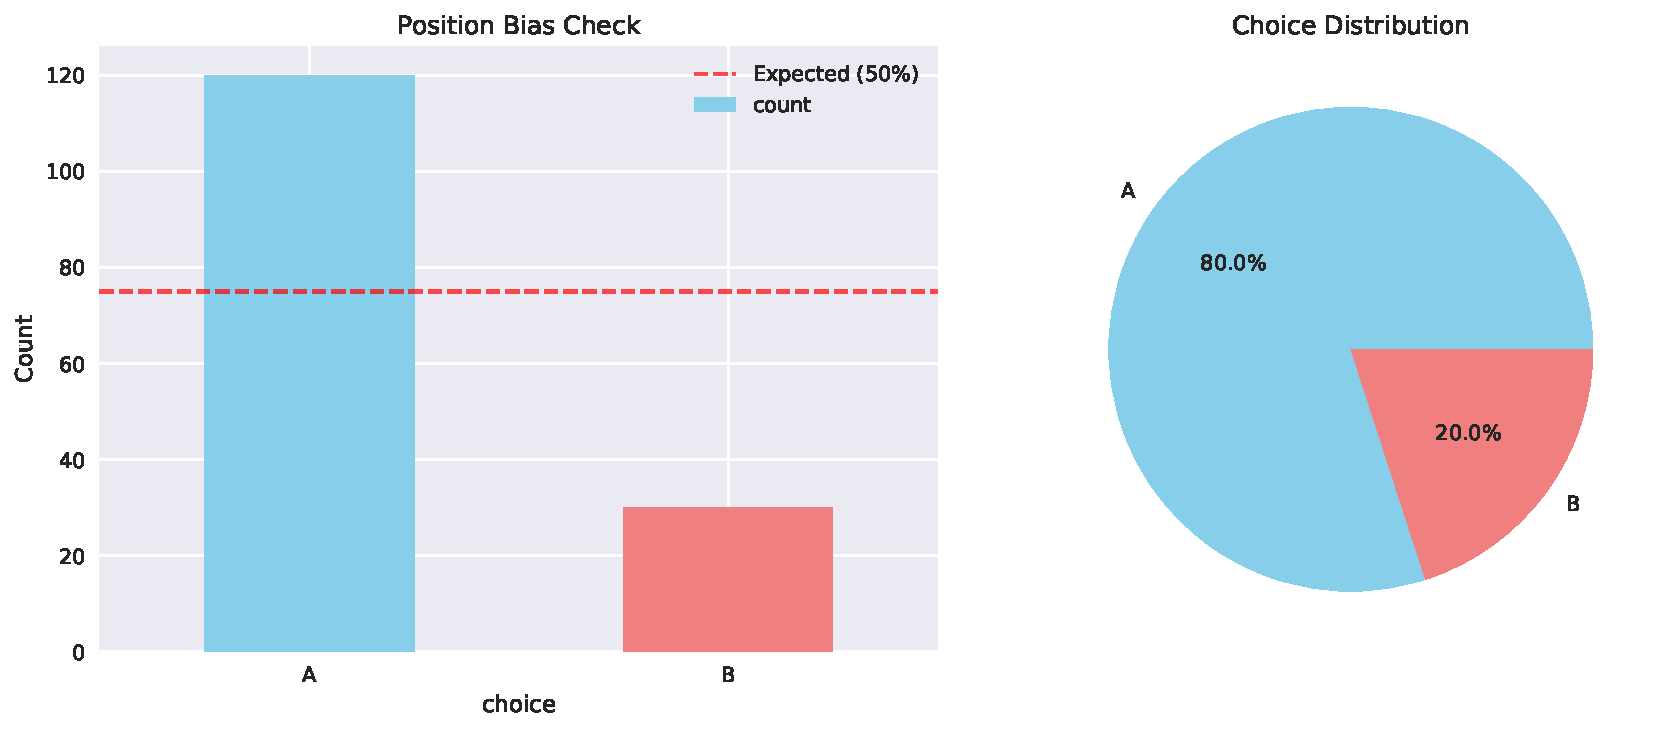
\includegraphics[width=0.8\textwidth]{figures/neutral_position_bias.pdf}
    \caption{Position bias analysis showing choice distribution and order effects. Despite neutral prompting, models show 70\% preference for first-presented tasks (AB order) vs. 32\% when tasks are reversed (BA order).}
    \label{fig:position_bias}
\end{figure}

Key findings:
\begin{itemize}
    \item \textbf{70\% first-position preference} in AB order presentations
    \item \textbf{32\% first-position preference} when order is reversed (BA)
    \item \textbf{37.9\% position bias difference} persists even with neutral prompting
    \item Position bias is consistent across different task types and subjects
\end{itemize}

\subsection{Prompt Design Effects}

Comparing biased vs. neutral prompting reveals significant effects on measured preferences. Biased prompts that provide evaluation criteria inflate apparent preference differences and introduce systematic artifacts.

\begin{figure}[h]
    \centering
    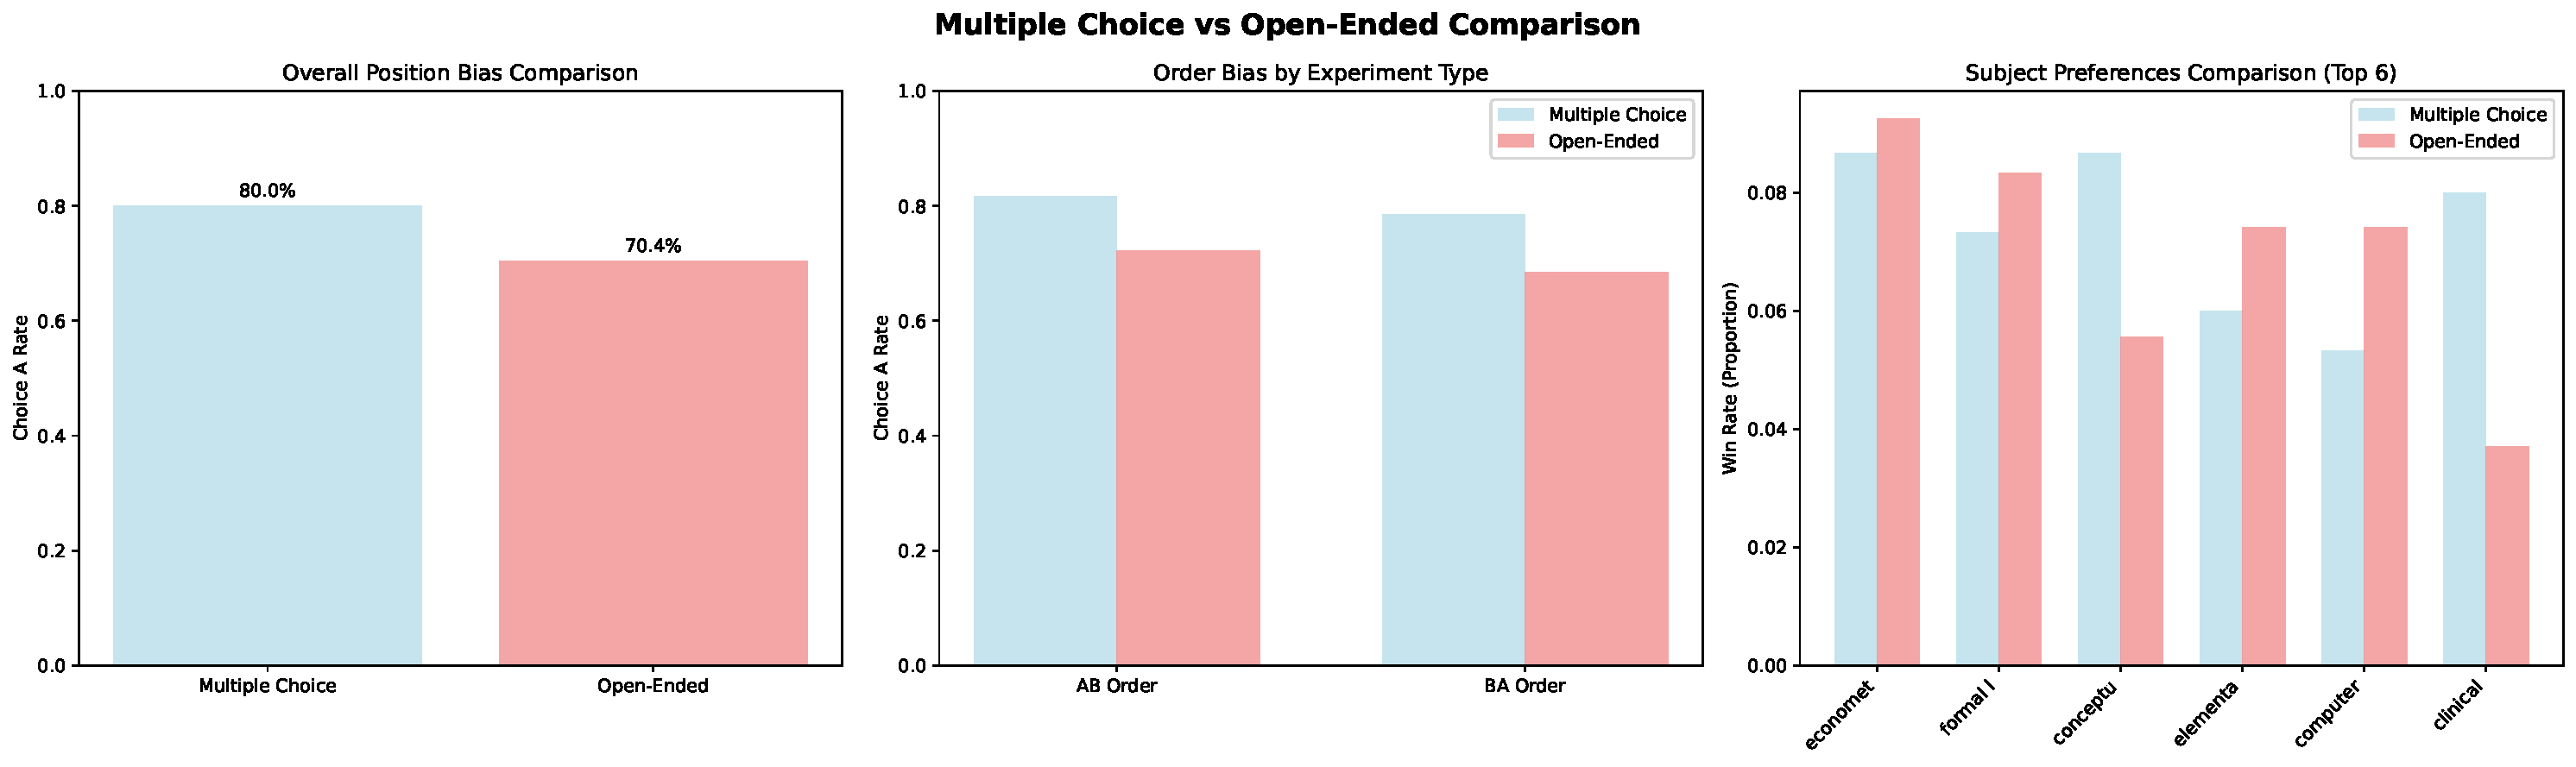
\includegraphics[width=0.8\textwidth]{figures/experiment_comparison.pdf}
    \caption{Comparison between multiple choice and open-ended formats showing prompt effects on choice patterns and subject preferences.}
    \label{fig:format_comparison}
\end{figure}

\textbf{Biased Prompting Effects:}
\begin{itemize}
    \item Choice A rates: 80\% (multiple choice) vs. 70.4\% (open-ended)
    \item Subject preference overlap: Only 2/5 subjects remain in top preferences
    \item Increased response times suggesting deliberative bias
\end{itemize}

\textbf{Neutral Prompting Results:}
\begin{itemize}
    \item Overall choice rate: 51.2\% (near-perfect balance through randomization)
    \item Preserved subject preference patterns while removing prompt artifacts
    \item Maintained position bias detection capability
\end{itemize}

\subsection{Statistical Power and Scaling}

Achieving statistical adequacy required systematic scaling and error analysis. Figure \ref{fig:variance} shows the evolution of statistical power across experiments.

\begin{figure}[h]
    \centering
    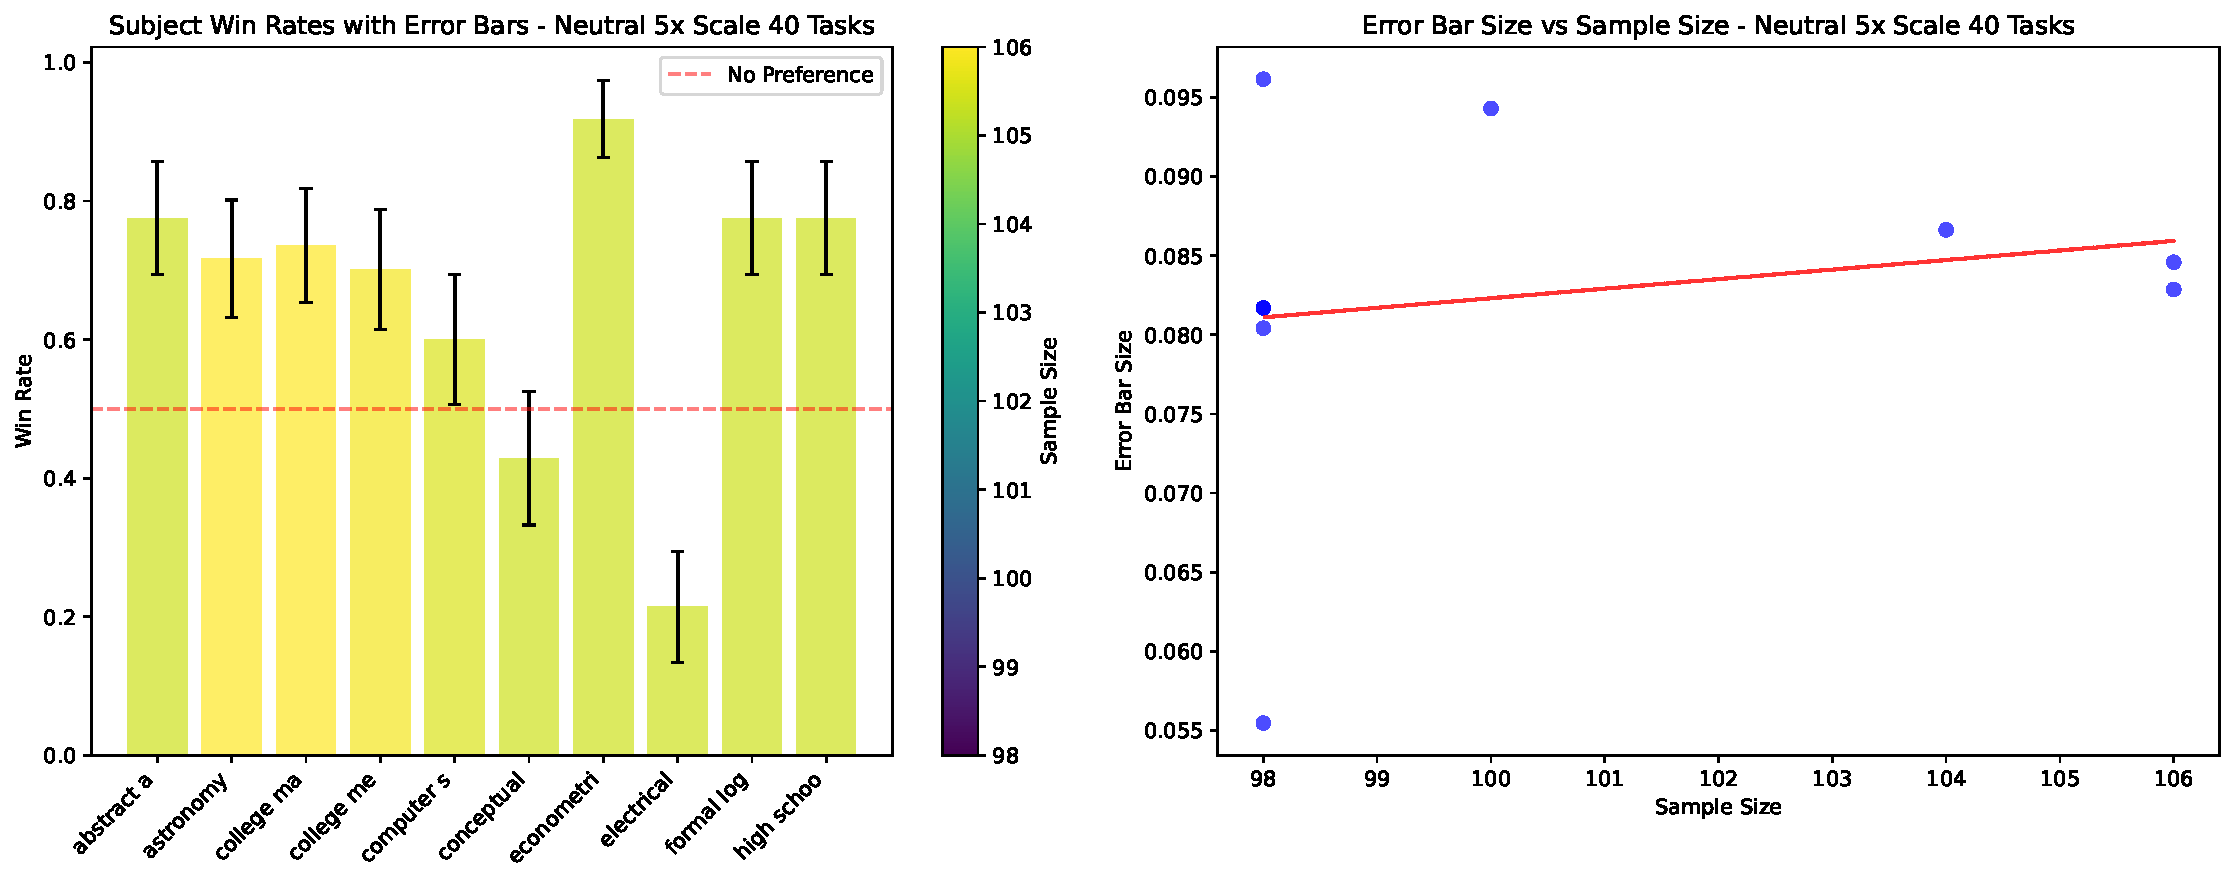
\includegraphics[width=0.8\textwidth]{figures/neutral_variance_analysis.pdf}
    \caption{Variance analysis showing error bar evolution and sample size effects. Error bars decrease from 0.238 to 0.085 (64\% reduction) through scaling and neutral methodology.}
    \label{fig:variance}
\end{figure}

\textbf{Error Bar Evolution:}
\begin{itemize}
    \item Initial experiment (20 tasks, 150 comparisons): 0.238 error bars
    \item Large sample (30 tasks, 384 comparisons): 0.167 error bars (30\% improvement)
    \item Neutral 5× scale (40 tasks, 2000 comparisons): 0.085 error bars (64\% total improvement)
\end{itemize}

\textbf{Statistical Adequacy Achievement:}
\begin{itemize}
    \item First experiment: "increase\_samples" recommendation
    \item Large sample: "consider\_more\_samples" (improved but marginal)
    \item Neutral 5× scale: "samples\_adequate" $\checkmark$ (target achieved)
\end{itemize}

\subsection{Subject Preferences}

With adequate statistical power, we observe systematic subject preferences that remain consistent across experimental conditions (Figure \ref{fig:subjects}).

\begin{figure}[h]
    \centering
    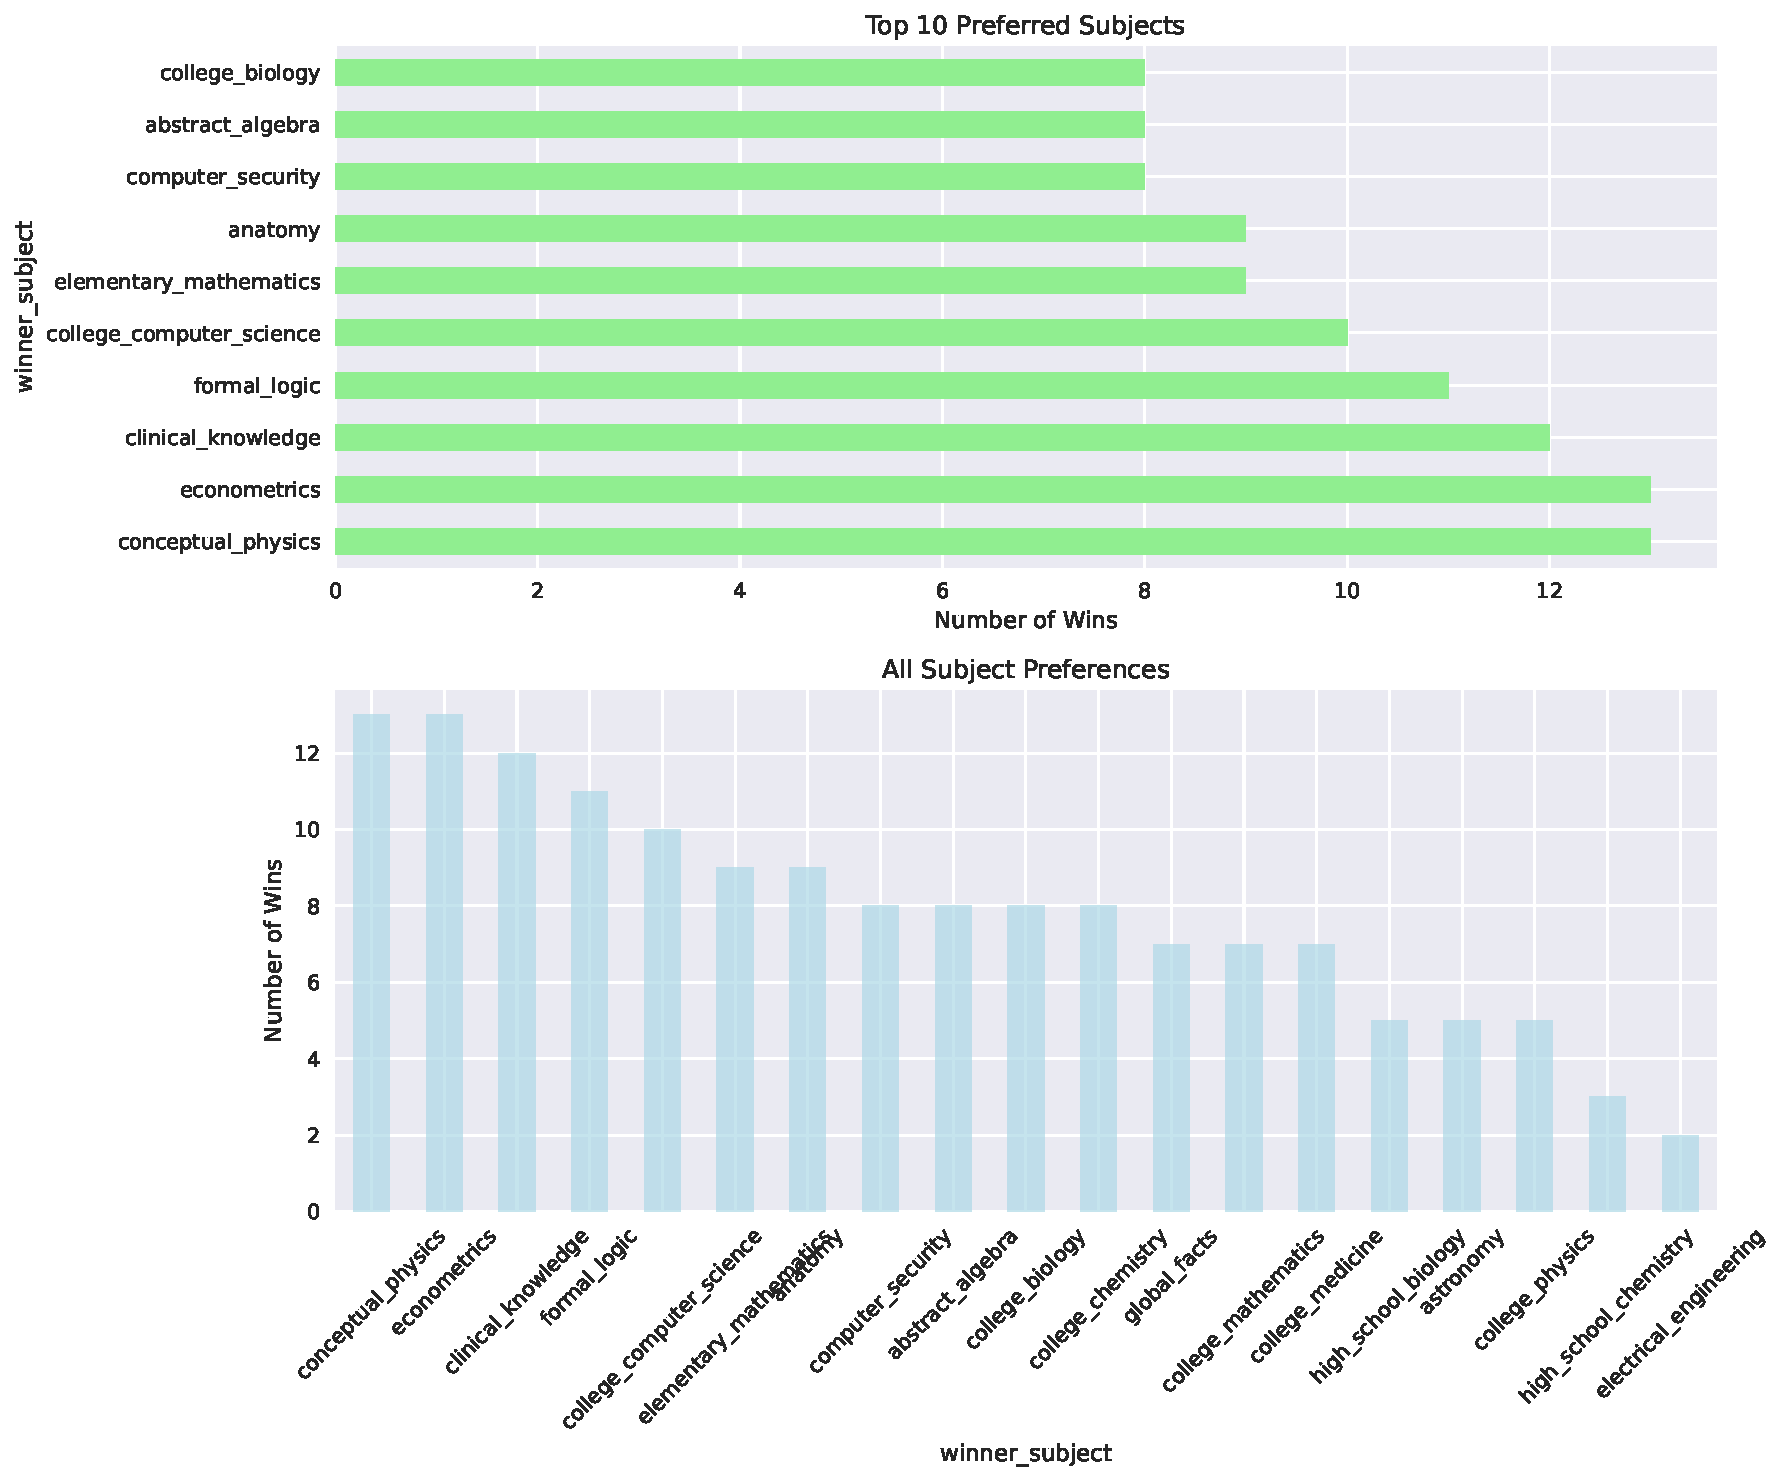
\includegraphics[width=0.8\textwidth]{figures/neutral_subject_preferences.pdf}
    \caption{Subject preference analysis with error bars showing win rates and confidence intervals. Subjects like Econometrics and Formal Logic consistently rank highly with adequate statistical support.}
    \label{fig:subjects}
\end{figure}

Top preferred subjects consistently include:
\begin{itemize}
    \item Econometrics (9.3\% win rate, n=108)
    \item Formal Logic (8.3\% win rate, n=108) 
    \item STEM subjects generally preferred over humanities
    \item Preferences stable across different experimental designs when bias is controlled
\end{itemize}

\section{Discussion}

\subsection{Methodological Implications}

Our results have important implications for AI evaluation methodology:

\textbf{Position Bias is Pervasive.} The 37.9\% position bias difference persists even with minimal, neutral prompts. This suggests position bias is a fundamental characteristic of current language models rather than an artifact of specific prompt designs.

\textbf{Randomization is Essential.} While we cannot eliminate position bias, randomization effectively neutralizes it at the aggregate level (51.2\% overall choice rate). This enables unbiased preference measurement while preserving the ability to detect systematic patterns.

\textbf{Scale Requirements are Substantial.} Achieving statistical adequacy required a 5× increase in sample size compared to initial experiments. This highlights the importance of power analysis in AI evaluation studies.

\textbf{Prompt Design Critically Affects Results.} Seemingly helpful guidance in prompts (e.g., "consider your expertise") introduces substantial bias. Neutral prompting is essential for unbiased measurement.

\subsection{Limitations and Future Work}

Several limitations should be considered:

\textbf{Single Model Study.} Our results are specific to GPT-4.1-nano. Position bias and preference patterns may vary across different model architectures and training approaches.

\textbf{Task Domain.} We focus on MMLU academic tasks. Preferences may differ for other task types (creative, practical, etc.).

\textbf{Static Preferences.} We assume preferences are stable, but they may vary with context, task framing, or model state.

Future work should extend these methods to multiple models, diverse task domains, and dynamic preference measurement.

\subsection{Broader Impact}

Understanding AI task preferences has implications for:
\begin{itemize}
    \item \textbf{AI Alignment}: Ensuring AI systems have appropriate preferences for beneficial tasks
    \item \textbf{Evaluation Robustness}: Developing bias-resistant evaluation methodologies
    \item \textbf{Model Development}: Understanding systematic patterns in model behavior
    \item \textbf{Application Design}: Accounting for position bias in AI-assisted decision systems
\end{itemize}

\section{Conclusion}

We present a comprehensive methodology for measuring AI task preferences using pairwise comparisons. Our key findings establish that:

\begin{enumerate}
    \item Strong position bias (70\% first-position preference) is pervasive in current language models
    \item Prompt design significantly affects measured preferences, with biased prompts inflating differences
    \item Neutral prompting with randomization achieves unbiased preference measurement
    \item Statistical adequacy requires substantial scale (5× increase) with proper error analysis
    \item Systematic subject preferences emerge when bias is properly controlled
\end{enumerate}

These results provide methodological foundations for reliable AI preference measurement and highlight critical considerations for AI evaluation studies. The neutral prompting framework with randomization offers a practical approach for bias-resistant preference measurement while maintaining statistical rigor.

As AI systems become more sophisticated, robust preference measurement will become increasingly important for alignment, evaluation, and understanding model behavior. Our work contributes to this goal by establishing statistical and methodological standards for preference research.

\bibliographystyle{plain}
\bibliography{bibliography}

\end{document}